\section{A Block Successive Over Relaxation Method}
\label{sec:block_sor}

Applying the Mat\'ern type prior covariance operator, $C$
requires the solution to an elliptic equation.
We outline here a block-Successive Over Relaxation (SOR) method that was
implemented to solve this problem.
We first make a few notes regarding why we chose this algorithm, and why it had
to be implemented at all.

For better or for worse, the MITgcm is a standalone package, and any code
modifications must not rely on outside packages in order to be incoroporated in
the main distribution.\footnote{The notable exception being the expensive,
    proprietary algorithmic differentiation software TAF \citep{giering2005}
    that is tightly interwoven into the code to enable the adjoint model.}
Therefore, incorporating a solver from e.g.\ \texttt{PETSc} is not allowed.
The MITgcm does contain a conjugate gradient solver, but this relies on
a preconditioning that is motivated by geophysical fluid dynamics that may not
be relevant to the more general Mat\'ern SPDE structure.
Thus, we use the SOR method as it is generally easy to implement, and is ``fast
enough'' noting that the computational cost of most elliptic solvers will be
inconsequential when compared to the time-dependent forward model.

The SOR method is an iterative method for solving $A\mathbf{x} = \mathbf{b}$.
At iteration $k$, the elements of $\mathbf{x}$ are $x_i^k$ (similar
notation for other variables), and we seek the update:
\begin{linenomath}\begin{equation}
    \tilde{x}_i^{k+1} = (1-\omega) x_i^k + \dfrac{\omega}{a_{ii}}
    \left( b_i - \sum_{j<i}a_{ij}\tilde{x}_j^{k+1} -
        \sum_{j>i}a_{ij}x_j^{k}\right), \qquad
        i=1,2,...,N \, ,
    \label{eq:sor_update}
\end{equation}\end{linenomath}
where $\omega$ is the SOR parameter.
We compare this method to the standard Jacobi update
\begin{linenomath*}\begin{equation*}
    \tilde{x}_i^{k+1} = x_i^k + \sum_{i\ne j}\dfrac{a_{ij}x_j^k}{a_{ii}},
    \qquad i=1,2,...,N \, .
\end{equation*}\end{linenomath*}
Here the notation $\tilde{x}_i^{k+1}$ refers to the fact this is a local update,
i.e. there is no communication between the processes assigned to each portion of
the computational domain.
The only areas where this local update causes the algorithm to deviate from a
true SOR method is where neighboring elements
$\tilde{x}^{k+1}_{j}, i\ne j$ are in the ``halo'' regions (i.e. outside of a
process's subdomain).
In this case, $\tilde{x}^{k+1}_j = x^k_j$.

\begin{figure}
    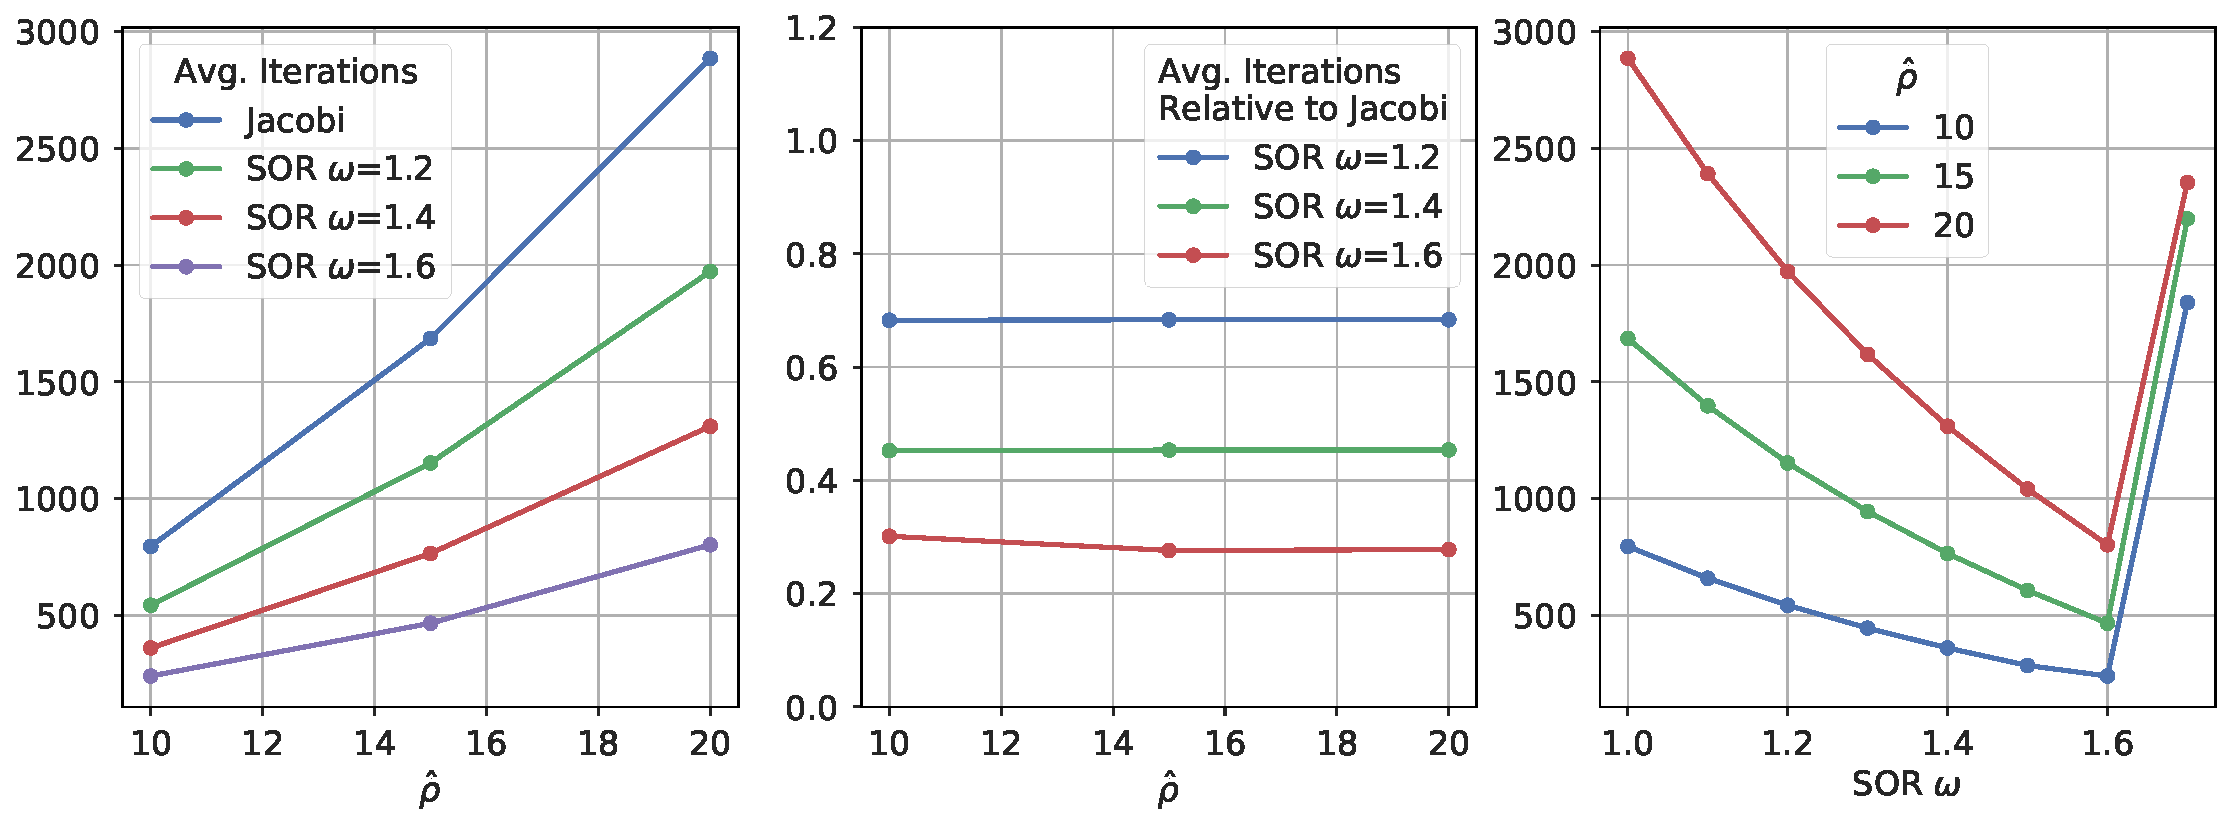
\includegraphics[width=\textwidth]{../figures/sor_noXi.pdf}
    \caption{Performance of the SOR algorithm for various settings of $\omega$.
        Average number of SOR or Jacobi iterations to convergence are shown
        based on solving equation \eqref{eq:fv_spde} with 1000 samples from a
        standard normal as the right hand side. Here $\xi=1$.}
    \label{fig:sor}
\end{figure}

We find this simple modification to be an effective means of speeding up the
linear solve.
Figure \ref{fig:sor} shows that the number of iterations required for
convergence is reduced to about 30\% of the Jacobi scheme.
Of course, a major drawback of the SOR algorithm is exhibited here as well: the
efficiency is highly sensitive to the parameter $\omega$, as shown in
right panel of Figure \ref{fig:sor}.
We
additionally find the performance to be dependent on the length scales used in the Jacobian
$\defjac$, defined in section \ref{sec:matern_operator}.
To facilitate the discussion, we define $L_y = \xi \Delta y$, where $\xi$ is
some multiple that accentuates length scales further in the meridional direction
(e.g.\ $\xi=2$ in many of the results shown in this work).
The vertical length scale is kept the same as before, i.e.\ $L_z = \Delta r$.
We report here that the optimal SOR parameter depends on $\xi$, as shown in
Figure \ref{fig:sor}, and
the optimal parameter for each $\xi$ tested is shown in
Table \ref{table:sor_xi}.
As $\xi$ increases, $\omega^*\rightarrow 1$, and the algorithm approaches
the standard Jacobi algorithm.

\begin{table}[]
    \centering
    \caption{Optimal SOR parameter $\omega^*$ as a function of
        $\xi$, where $L_y = \xi \Delta y$.}
    \label{table:sor_xi}
    \begin{tabular}{c|c|c|c|c}
                   & $\xi=1/2$ & $\xi=1$ & $\xi=2$ & $\xi=5$ \\ \hline
        $\omega^*$ & 1.8 & 1.6 & 1.3 & 1.2                   \\
\end{tabular}
\end{table}

Finally, we note that in the current implementation of this algorithm we update
the ``halo'' regions of $\x$, i.e. $\tilde\x\rightarrow\x$, at the end of each iteration in the
solver.
We recognize that performance could be improved further by
increasing the number of iterations taken before updating the halo regions,
in to reduce communication.
This possible performance benefit could be explored in future work.
